\documentclass{ug}
\usepackage{float}
\usepackage{color, colortbl}
\usepackage[section]{placeins}
\usepackage{mathtools}
\usepackage{amsthm}
%\usepackage[T1]{helvet}
\usepackage[OT1]{fontenc} 


\theoremstyle{plain}
\newtheorem*{defn*}{Definition}
\newtheorem*{ex*}{Example}

\definecolor{iob-green}{rgb}{0.0,1.0,0.80}
\definecolor{iob-blue}{rgb}{0.90196,0.94902,1}

\title{IObundle 2ES MP3 Encoder}

\category{User Guide}

\begin{document}
\maketitle
\cleardoublepage
\tableofcontents
\cleardoublepage
\listoftables
\cleardoublepage
\listoffigures
\cleardoublepage

\section*{Revision History}

\begin{table}[H]
  \begin{center}
    \begin{tabular}{|l|l|p{8cm}|}
      \hline
      \rowcolor{iob-green}
      \textbf{Date} & \textbf{Author} & \textbf{Summary of changes} \\
      \hline
      \hline

      15/06/2018 & J. Sousa & Initial draft \\
      \hline

      \rowcolor{iob-blue} 19/06/2018 & J. Sousa & Added revision history. Added
      second mute signal in Table~\ref{tab:is}. Improved
      Table~\ref{tab:spi-args}, removed direct setting or getting of Control
      Word. Added Table~\ref{tab:spi-resp}. Added Table~\ref{tab:consts}.  Added
      Timing column to Table~\ref{tab:status}.\\ \hline

      20/06/2018 & J. Sousa & Improved Fig.~\ref{fig:fchart},
      Table~\ref{tab:res}, removed FIFO status bits and improved
      table~\ref{tab:status}, added Table~\ref{fig:out}, improved
      Fig.~\ref{fig:spi}, added section.\\ \hline

      \rowcolor{iob-blue} 21/06/2018 & J. Sousa & Changed document category to
      User Guide, improved Fig.~\ref{fig:fchart}, added signals in
      Table~\ref{tab:status}, added Fig.~\ref{fig:out}, UART reference, second
      watchdog timer for system stall.\\ \hline

      22/06/2018 & J. Sousa & Hided hyperlink color borders, improved
      Fig.~\ref{fig:bd}, Added RS232 and channel mode to features. Improved
      Fig.~\ref{fig:out}. Removed white spaces. Added HW and SW hard coded
      version parameters. Improved Table~\ref{tab:freq}.\\ \hline

      \rowcolor{iob-blue} 23/06/2018 & J. Sousa & Pause mode added. Fixed
      tables~\ref{tab:out}, \ref{tab:spi-args}, \ref{tab:spi-ctr}
      \ref{tab:spi-resp}, \ref{tab:status}, \ref{tab:intrrpt}, \ref{tab:freq}.
      Table~\ref{tab:cdc} added. Fixed Figs.~\ref{fig:bd} and
      \ref{fig:fchart}.\\ \hline

      25/06/2018 & J. Sousa & Stop command removed. Reset and pause commands
      improved.  Fixed tables~\ref{tab:is}, \ref{tab:spi-cmd},
      \ref{tab:spi-resp}, \ref{tab:intrrpt}, \ref{tab:freq}.  Explanation added
      in section~\ref{sec:cdc}. Fixed Figs.~\ref{fig:spi},
      \ref{fig:fchart}. Replaced T\_com with T\_cmd.\\ \hline

      \rowcolor{iob-blue} 27/06/2018 & J. Sousa & Improved
      Fig.~\ref{fig:spi}. Added conversion formula after
      Table~\ref{tab:consts}. Created a clear separation in
      Table~\ref{tab:spi-resp}. Added explanation in Table~\ref{tab:spi-args}.
      Created split tables \ref{tab:status} and \ref{tab:intrrpt}. Added
      section~\ref{sec:intrrptMask} that describes the mask bits. Added
      section~\ref{sec:wtd}. Added section~\ref{sec:lat}. Added
      Table~\ref{sec:lat}. Updated RS232 usage.\\ \hline

      28/06/2018 & J. Sousa & Improved Fig.~\ref{fig:i2s} and \ref{fig:bd},
      Tables~\ref{tab:intrrpt} and \ref{tab:cdc}, section~\ref{sec:wtd},
      \ref{sec:lat}, \ref{sec:intrrptact}. \\ \hline

      \rowcolor{iob-blue} 29/06/2018 & J. Sousa & Added Table~\ref{tab:si} and improved
      Table~\ref{tab:out}, Table~\ref{tab:status}, Table~\ref{tab:intrrpt},
      Table~\ref{tab:spi-cmd}, Table~\ref{tab:freq}, Table~\ref{tab:out},
      Fig.~\ref{fig:out}, Fig.~\ref{fig:fchart}, Table~\ref{tab:res},
      Table~\ref{tab:spi-ctr}, Table~\ref{tab:spi-args}.\\ \hline

      09/07/2018 & J. Sousa & Removed 24-bit support and added sample
      rate conversion table.\\ \hline

      \rowcolor{iob-blue} 11/07/2018 & J. Sousa & Fixed Fig.~\ref{fig:bd},
      Table~\ref{tab:out}, Table~\ref{tab:res}.\\ \hline

      12/07/2018 & J. Sousa & Improved
      tables~\ref{tab:is}, \ref{tab:is}, \ref{tab:is}, \ref{tab:si},
      \ref{tab:status}, \ref{tab:intrrpt}, \ref{tab:src}.  Added
      tables~\ref{tab:rs232},\ref{tab:cpu0_status_interrpt}. Replaced
      watchdog timer table with plain text explanation. Removed fixed
      sample rate from Fig.~\ref{fig:out}\\ \hline
      
    \end{tabular}
    \caption{Revision history}
  \end{center}
\end{table}
\clearpage


\begin{table}[H]
  \begin{center}
    \begin{tabular}{|l|l|p{8cm}|}
      \hline
      \rowcolor{iob-green}
      \textbf{Date} & \textbf{Author} & \textbf{Summary of changes} \\
      \hline
      \hline
      
     23/07/2018 & J. Sousa & Fixed Table~\ref{tab:src} and
     Table~\ref{tab:res}. Added clarification on latency. Added
     correct part number to block diagram.\\ \hline

     \rowcolor{iob-blue} 25/07/2018 & J.  Sousa & Added symbol in
     Fig.~\ref{fig:symb}. Added Ethernet interface signals and explanations. All
     SPI operation material grouped in section~\ref{sec:spi} and detailed
     comments to each subsection. Added Ethernet testing.\\ \hline

     26/07/2018 & J. Sousa & Fixed this table. Fixed
     section~\ref{sec:intrrptMask}. Improved Fig.~\ref{fig:bd}. Added
     section~\ref{sec:func}. Added correct part number to
     Table~\ref{tab:res}.\\ \hline

     \rowcolor{iob-blue} 28/07/2018 & J. Sousa & Replaced Intel Ethernet core with
     IObundle 2-port UDP core. Improved explanation for Reset command
     and recommended action on Stall. Renamed InvalidCommand to
     cmdFail and moved this interrupt flag from CPU1/2 to
     CPU0.\\ \hline
    
     31/07/2018 & J. Sousa & Replaced Ethernet IP
     in features and its section.\\ \hline

     \rowcolor{iob-blue} 27/08/2018 & J. Sousa & Changed Fig.~\ref{fig:bd},
     Fig.~\ref{fig:spi}, section~\ref{sec:bd}, section~\ref{sec:spi}\\ \hline

     09/09/2018 & J. Sousa & Updates figures: \ref{fig:bd}, \ref{fig:i2s},
     \ref{fig:out}, \ref{fig:fchart}. Updated tables: \ref{tab:consts},
     \ref{tab:is}, \ref{tab:rs232}, \ref{tab:i2s}, \ref{tab:out},
     \ref{tab:spi-args}, \ref{tab:spi-resp}, \ref{tab:intrrpt},
     \ref{tab:intrrptMask}, \ref{tab:res}. Added
     section~\ref{sec:rates}\\ \hline

     \rowcolor{iob-blue} 17/09/2018 & J. Sousa & Added test section. Updated
     sections~\ref{sec:func}.\\ \hline

     01/05/2019 & J. Sousa & Complete user guide upgrade. Removed Ethernet and
     testing sections.\\ \hline

     \rowcolor{iob-blue} 09/06/2019 & J. Sousa & Changed timeout and interrupt
     mask defaults and changed returned SIW upon RUN, RESET and PAUSE.\\ \hline

     28/08/2019 & J. Sousa & User guide update. Added HALF\_VOLUME
     parameter. Updated FPGA implementation results. Improved features. Fixed
     block diagram and module explanation. Removed I2S underflow flag. Improved
     Latency section. Improved flow chart and added explanation on the bitrate
     change procedure.\\ \hline

    \end{tabular}
    \caption{Revision history (continued)}
  \end{center}
\end{table}
\clearpage




\section*{Constants}

\begin{table}[H]
  \begin{center}
    \begin{tabular}{|c|c|c|p{7cm}|}
      \hline
      \rowcolor{iob-green}
      \textbf{Symbol} & \textbf{Value} & \textbf{Unit} & \textbf{Description} \\
      \hline
      \hline

      $f_{sys\_clk}$ & User specified & Hz & System clock frequency
      \\ \hline

      \rowcolor{iob-blue}
      $f_{sample}$ & 48 & kHz & Sample rate frequency \\
      \hline

      $f_{i2s\_lrclk}$ & 48 & kHz & Audio input I2S word clock
      frequency \\ \hline

      $f_{spi\_sclk}$ & User specified & Hz & SPI interface clock
      frequency\\ \hline

      \rowcolor{iob-blue} $f_{out\_clk}$ & User specified & kHz &
      Audio output parallel interface clock\\ \hline

      $l_{frame}$ & 576 or 1152 & none & PCM frame duration in
      samples. 576 samples for 32 and 64 kbps bitrates due to internal
      sample rate conversion to 16 and 24 kHz, respectively \\ \hline

      \rowcolor{iob-blue} $T_{cmd}$ & 10000 & System clock cycles &
      Guaranteed max time to process a command \\ \hline

    \end{tabular}
    \caption{Table of constants}
    \label{tab:consts}
  \end{center}
\end{table}

\clearpage

\section{Introduction}

The IOB-2ES-MP3-E is an IP core for independent and simultaneously encoding 2
audio PCM streams into 2 MPEG 1/2 Layer III (MP3) audio streams. The IP is
currently supported in Intel FPGAs.


\subsection{Symbol}

\begin{figure}[h]
  \begin{center}
    \includegraphics[width=12cm]{symb.png}
    \caption{IP symbol}
    \label{fig:symb}
  \end{center}
\end{figure}
\clearpage

\subsection{Features}

\begin{itemize}
\item ISO/IEC 11172-3 MPEG 1 Layer III standard
\item SPI slave interface for configuration, control and status information
\item RS232 interfaces for viewing runtime messages
\item 2 encoder CPUs
\item 1 control CPU
\item 1 SPI interface for system control 
\item 2 Audio input I2S slave interfaces
\item 2 Audio output parallel master interfaces
\item 48KHz audio sample rate frequency
\item Supported bitrates: 32, 64, 128 and 192 kbps
\item Internal sample rate converter applied for bitrates 32 kbps (input
  converted to 16KHz) and 64 kbps (input converted to 24KHz)
\item 16-bit audio sample size
\item Fixed stereo audio channel mode
\item 2-frame latency (from first sample in to first byte out)
\item Real time operation at 90MHz
\item 3 watchdog timers to detect stall in each CPU
\item -6dB volume control
\end{itemize}

\subsection{Benefits}
\begin{itemize}
\item Compact hardware implementation
\item Can be integrated with other functions in the same FPGA
\item Low operation frequency
\item Low power consumption
\end{itemize}

\clearpage

\section{Block Diagram}
\label{sec:bd}

\begin{figure}[h]
  \begin{center}
    \includegraphics[width=16cm]{bd.png}
    \caption{Block diagram}
    \label{fig:bd}
  \end{center}
\end{figure}
\clearpage

\subsection{Functional Description}
\label{sec:func}

\subsubsection{Hardware Components}

The hardware modules below have been developed by IObundle Lda by default. Some
modules are Intel IP and are indicated below.

\begin{description}
\item {\bf MP3-FE}: MP3 front-end (sample rate conversion, sub-band filter bank
  and MDCT) implemented using the CGRA-V architecture, owned by IObundle, Lda.
\item {\bf SPI slave}: Used for receiving commands from host machine.
\item {\bf I2S IN}: Used by CPU1 and CPU2 to input PCM audio data.
\item {\bf I2S OUT}: Used by CPU0 to produce a test I2S interface
\item {\bf PAR OUT}: Used by CPU1 and CPU2 to output MP3 audio data.
\item {\bf PAR IN}: Used by CPU0 to input MP3 audio data for testing.
\item {\bf Control, Status \& Interrupt}: Used by CPU0 to send commands to CPU1
  and CPU2, used by the 3 CPUs to update status and interrupt bits.
\item {\bf NIOS II/f CPU0}: Used for system control and test. Controls CPU1 and
  CPU2 according to user commands. Receives commands and sends
  responses via SPI. Updates its status and interrupt bits. (Intel IP)
\item {\bf NIOS II/f CPU1 and CPU2}: Used for encoding audio data in the MP3
  format. Receive commands and encoding parameters from CPU0 via Control
  Reg. Receive data from Audio IN I2S and send encoded data through Audio OUT
  PAR. Update their status and interrupt bits. (Intel IP)
\item {\bf RS232}: Used for displaying runtime messages, errors and status
  information. (Intel IP)
\item {\bf Watchdog}: Used to monitor if the respective host CPU has
  stalled. (Intel IP)
\end{description}

\subsubsection{Software Components}

\begin{description}
\item {\bf IOB-MP3}: MP3 encoder wrapper: controls and configures the
  libSHINE encoder library according to commands received from
  IOB-MP3-CTR. Runs on CPU1 and CPU2.
\item {\bf IOB-MP3-CTR}: Runs on CPU0 and controls and configures the
  encoders running on CPU1 and CPU2.
\item {\bf libSHINE}: MP3 encoder library. Called by IOB-MP3. Available from
  \url{https://github.com/toots/shine}
\end{description}

\section{Interface Signals}

\subsection{General Interface Signals}

\begin{table}[H]
  \begin{center}
    \begin{tabular}{|l|l|p{8cm}|}
      \hline
      \rowcolor{iob-green}
      \textbf{Signal} & \textbf{Direction} & \textbf{Description} \\
      \hline
      \hline

      sys\_clk &  IN & Main system clock \\
      \hline

      \rowcolor{iob-blue} sys\_rst & IN & Asynchronous active high reset
      signal. \\ \hline

      mute\_1 & IN & When high mutes encoder on CPU1. I2S input data
      is ignored and a muted MP3 stream is produced at the
      output. \\ \hline

      \rowcolor{iob-blue}
      mute\_2 & IN & When high mutes encoder on CPU2. I2S input data
      is ignored and a muted MP3 stream is produced at the
      output. \\ \hline

      interrupt & OUT & Interrupt signal; goes high if any
      unmasked interrupt bit is high.\\ \hline

      status[31:0] & OUT & Status and Interrupt Word as in Table~\ref{tab:si}.\\ \hline

    \end{tabular}
    \caption{General interface signals}
    \label{tab:is}
  \end{center}
\end{table}

\subsection{RS232 Interface Signals}

The RS232 IP core used in the {\it Intel FPGA UART Core} described in Chapter 9
of the following document accessed in June/20/2018 from

\hyperlink{https://www.altera.com/en\_US/pdfs/literature/ug/ug\_embedded\_ip.pdf}{https://www.altera.com/en\_US/pdfs/literature/ug/ug\_embedded\_ip.pdf}.

Three instances of this IP are being used, one for each CPU. However, only one
RS232 pin is used, according to the table below:

\begin{table}[H]
  \begin{center}
    \begin{tabular}{|l|l|p{8cm}|}
      \hline
      \rowcolor{iob-green}
      \textbf{Signal} & \textbf{Direction} & \textbf{Description} \\
      \hline
      \hline

      rs232\_tx &  OUT & Serial transmit signal from CPU0\\
      \hline

      rs232\_tx\_1 &  OUT & Serial transmit signal from CPU1\\
      \hline

      rs232\_tx\_2 &  OUT & Serial transmit signal CPU2\\
      \hline

    \end{tabular}
    \caption{RS232 interface signals}
    \label{tab:rs232}
  \end{center}
\end{table}
\clearpage

\subsection{Audio Input I2S Slave Interface}

\begin{table}[H]
  \begin{center}
    \begin{tabular}{|l|l|l|}
      \hline
      \rowcolor{iob-green}
      \textbf{Signal} & \textbf{Direction} & \textbf{Description} \\
      \hline
      \hline

      i2s\_bclk\_1 & IN & Bit clock for encoder on CPU1. Samples data at rising edge.\\
      \hline

      \rowcolor{iob-blue}
      i2s\_lrclk\_1 & IN & Word clock for encoder on CPU1. Left channel when 0, right when 1.\\
      \hline

      i2s\_data\_1 & IN & I2S serial data for encoder on CPU1.\\
      \hline
      \hline

      i2s\_bclk\_2 & IN & Bit clock for encoder on CPU2. Samples data at rising edge.\\
      \hline

      \rowcolor{iob-blue}
      i2s\_lrclk\_2 & IN & Word clock for encoder on CPU2. Left channel when 0, right when 1.\\
      \hline

      i2s\_data\_2 & IN & I2S serial data for encoder on CPU2.\\
      \hline

    \end{tabular}
    \caption{Audio input I2S slave interface}
    \label{tab:i2s}
  \end{center}
\end{table}



\subsection{Audio Output Parallel Interface}

\begin{table}[H]
  \begin{center}
    \begin{tabular}{|l|l|p{8cm}|}
      \hline
      \rowcolor{iob-green}
      \textbf{Signal} & \textbf{Direction} & \textbf{Description} \\
      \hline
      \hline

      out\_clk & IN & Audio output clock.\\ \hline

      \rowcolor{iob-blue} out\_valid\_1 & OUT & Audio output valid for CPU1. \\ \hline
      
      out\_frame\_start\_1 & OUT & High when the first stream byte is output by CPU1, low
      otherwise.\\ \hline

      \rowcolor{iob-blue} out\_frame\_end\_1 & OUT & High when the last stream byte
      is output by CPU1, low otherwise.\\ \hline

      out\_bitrate\_1[1:0] & OUT & Audio output bit rate for CPU1: 00=32kbps,
      01=64kbps, 10=128kbps, 11=192kbps.\\ \hline

      \rowcolor{iob-blue}
      out\_samplerate\_1[1:0] & OUT & Audio output sample rate by CPU1: 00=16kHz,
      01=24kHz, 10=48kHz, 11=unused.\\ \hline

      out\_data\_1[7:0] & OUT & Audio output bistream data from CPU1 organized in bytes.\\
      \hline
      \hline

      \rowcolor{iob-blue} out\_valid & OUT & Audio output valid for CPU2. \\ \hline
      
      out\_frame\_start\_2[1:0] & OUT & High when the first stream byte is output by CPU2, low
      otherwise.\\ \hline

      \rowcolor{iob-blue} out\_frame\_end\_2[1:0] & OUT & High when the last stream byte
      is output by CPU2, low otherwise.\\ \hline

      out\_bitrate\_2[1:0] & OUT & Audio output bit rate for CPU2: 00=32kbps,
      01=64kbps, 10=128kbps, 11=192kbps.\\ \hline

      \rowcolor{iob-blue}
      out\_samplerate\_2[1:0] & OUT & Audio output sample rate for CPU2: 00=16kHz,
      01=24kHz, 10=48kHz, 11=unused.\\ \hline

      out\_data\_2[7:0] & OUT & Audio output bistream data  from CPU2 organized in bytes.\\
      \hline

    \end{tabular}
    \caption{Audio Output parallel interface signals}
    \label{tab:out}
  \end{center}
\end{table}


      
\subsection{SPI Slave Interface}

\begin{table}[H]
  \begin{center}
    \begin{tabular}{|l|l|l|}
      \hline

      \rowcolor{iob-green}
      \textbf{Signal} & \textbf{Direction} & \textbf{Description} \\
      \hline
      \hline

      spi\_sclk & IN & SPI serial (bit) clock.\\ \hline

      \rowcolor{iob-blue} spi\_mosi & IN & SPI master output / slave
      input.\\ \hline

      spi\_miso & OUT & SPI master input / slave output.\\ \hline

      \rowcolor{iob-blue} spi\_ss & IN & SPI slave select. \\ \hline

    \end{tabular}
    \caption{SPI slave interface}
    \label{tab:spi}
  \end{center}
\end{table}

\begin{figure}[H]
  \begin{center}
    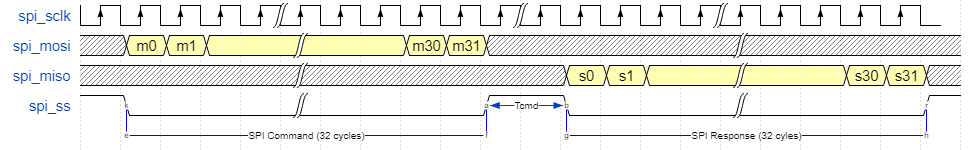
\includegraphics[width=16cm]{spi.png}
    \caption{SPI slave interface timing diagram}
    \label{fig:spi}
  \end{center}
\end{figure}


\section{SPI Operation}
\label{sec:spi}

\subsection{Master Control Word}

The Master Control Word (MCW) is sent by the SPI master to CPU0, in order to
control the operation of the IOB-2ES-MP3-E core. The structure of the MCW is
detailed in Fig.~\ref{tab:spi-ctr}.

\begin{table}[H]
  \begin{center}
    \begin{tabular}{|l|l|l|}
      \hline
      \hline
      \rowcolor{iob-green}
      \textbf{Command[31:28]} & \textbf{Processors[27:24]}  & \textbf{Argument[23:0]} \\
      \hline
      \hline
    \end{tabular}
    \caption{Master Control Word}
    \label{tab:spi-ctr}
  \end{center}
\end{table}

The MCW fields are described in the next subsections.

\clearpage 

\subsubsection{Command Field}

The list of commands that can be sent to the IOB-2ES-MP3-E core is
detailed in Table~\ref{tab:spi-cmd} below.

\begin{table}[H]
  \begin{center}
    \begin{tabular}{|l|l|p{12cm}|}
      \hline
      \rowcolor{iob-green}
      \textbf{Command} & \textbf{Code} & \textbf{Description} \\
      \hline
      \hline

      \textit{Get} & 0010 & Gets parameters according to the Argument field for
      the selected processor in the Processors field. It is possible to Get
      parameters for a running, paused or idle processor. The Processors field
      must select a single processor or otherwise the command is invalid and
      will raise the cmdFail interrupt bit.\\ \hline
      \rowcolor{iob-blue} \textit{Set} & 0001 & Sets parameters according to the
      Argument field for the selected processors in the Processors field. It is
      possible to Set parameters for an idle processor. Additionally, it is
      possible to Set the BIT\_RATE parameter for a running or paused processor,
      which becomes effective for encoding the next frame after the Set command
      is executed.\\ \hline

      \textit{Run} & 0011 & Runs the encoder processors selected in the
      Processors field. The command will enable the I2S input previously
      disabled. It is still possible to Get parameters for a running processor;
      however only the BIT\_RATE parameter can be set and any attempt to Set
      other parameters will raise the cmdFail interrupt bit. Argument
      field ignored.\\ \hline

      \rowcolor{iob-blue} \textit{Pause} & 0100 & Pauses the processors selected
      in the Processors field after finishing encoding the current
      frame. Settings, internal data buffers, input and output FIFOs are
      preserved. Data input is ignored. Argument field ignored.\\ \hline

      \textit{Reset} & 0000 & Sends a hardware reset to the processors selected
      in the Processors field. Restores parameters to default values. Flushes
      internal data buffers, input and output FIFOs. Resets the program
      counter. Status and interrupt bits are cleared. Namely, the Ready status
      bit of the selected processors goes low until this command has completed
      after which it goes high again. Argument field ignored.\\ \hline

    \end{tabular}
    \caption{Command field}
    \label{tab:spi-cmd}
  \end{center}
\end{table}

\subsubsection{Processors Field}

It is possible to send the same command to multiple processors by simultaneously
activating multiple bits of the Processors field.

\begin{table}[H]
  \begin{center}
    \begin{tabular}{|c|l|}
      \hline
      \rowcolor{iob-green}
      \textbf{Bit\#}  & \textbf{Description} \\
      \hline
      \hline

      27 & Reserved.\\ \hline

      \rowcolor{iob-blue} 26 & When high selects processor CPU2.\\ \hline

      25 & When high selects processor CPU1.\\ \hline

      \rowcolor{iob-blue} 24 & When high selects processor CPU0.\\ \hline

    \end{tabular}
    \caption{Processors field}
    \label{tab:spi-proc}
  \end{center}
\end{table}

\clearpage


\subsubsection{Argument Field}

The Argument field is used to send command options as explained in Table~\ref{tab:spi-args} below.

\begin{table}[H]
  \begin{center}
    \begin{tabular}{|l|l|c|p{7cm}|}
      \rowcolor{iob-green}
      \hline \textbf{Command} & \textbf{Parameter} & \textbf{Argument[23:16]} & \textbf{Argument[15:0]} \\
      \hline
      \hline

      \textit{Get} & BIT\_RATE(1)  & 0x04  & Don't Care. \\
      \hline
      
      \rowcolor{iob-blue}
      \textit{Get} & INTRRPT\_MASK & 0x05  &  Don't Care. \\
      \hline 

      \textit{Get} & STATUS\_INTRRPT & 0x0D & Don't Care. \\
      \hline 

      \rowcolor{iob-blue}
      \textit{Get} & TIMEOUT & 0x13 & Don't Care.  \\
      \hline 

      \textit{Get} & VERSION & 0x09 & Don't Care.\\
      \hline

      \rowcolor{iob-blue}
      \textit{Get} & LAST\_COMMAND & 0x12 & Don't Care.\\
      \hline
      \hline
      \hline

      \textit{Get} & HALF\_VOLUME & 0x0C & Don't Care.\\
      \hline
      \hline
      \hline

      \rowcolor{iob-blue}
      \textit{Set} & HALF\_VOLUME & 0x0C & 0 means full scale volume, non-zero
      means half scale volume (-6dB)\\ \hline

      \textit{Set} & TIMEOUT\_H & 0x01 & 16-bit high part of 32-bit
      system wait time limit to activate Stall in
      Table~\ref{tab:cpu0_status_interrpt} and Table~\ref{tab:intrrpt}
      given in system clock cycles.\\ \hline

      \rowcolor{iob-blue} \textit{Set} & TIMEOUT\_L & 0x02 & 16-bit low part of
      32-bit TIMEOUT parameter.\\ \hline

      \textit{Set} & BIT\_RATE & 0x04 & Output bitstream bit rate in
      kbps.  Valid settings are 0x0020 (32kpbs), 0x0040 (64kbps),
      0x0080 (128kbps) and 0x00C0 (192kbps).\\ \hline

      \rowcolor{iob-blue} \textit{Set} & INTRRPT\_MASK\_H & 0x06 & 16-bit high
      part of 32-bit Interrupt Mask Word. A bit is masked if its mask is 1 and
      unmasked otherwise.\\ \hline

      \textit{Set} & INTRRPT\_MASK\_L & 0x07 & 16-bit low
      part of 32-bit Interrupt Mask Word.  A bit is masked if its mask is 1 and
      unmasked otherwise.\\ \hline

      \rowcolor{iob-blue} \textit{Set} & INTRRPT\_CLR & 0x0F & Don't Care; clears
      the Interrupt Bits.\\ \hline

      \textit{Run}(2) & NA & Don't Care & Don't Care. \\ \hline

      \rowcolor{iob-blue} 
      \textit{Pause} & NA & Don't Care & Don't Care.\\ \hline

      \textit{Reset} & NA & Don't Care & Don't Care.\\ \hline

    \end{tabular}
    \caption{Argument field}
    \label{tab:spi-args}
  \end{center}
  (1) This Get command can only select one CPU, either CPU1 or
  CPU2. Otherwise the command will fail.

  (2) The Run command can only select CPU1, CPU2 or both but not
  CPU0. Selecting CPU0 will raise the CmdFail flag.
\end{table}

\clearpage

\subsection{Slave Response Word}

The Slave Response Word (SRW) is sent by CPU0 to the SPI master as
response to the previous command. For that the SPI master can
optionally perform an SPI read cycle after the write cycle to send the
command. See the timing diagram in Fig.~\ref{fig:spi}. The structure
of the SRW is detailed in Table~\ref{tab:spi-resp}.

\begin{table}[H]
  \begin{center}
    \begin{tabular}{|l|l|p{7cm}|c|}
      
      \rowcolor{iob-green}
      \hline \textbf{Command} & \textbf{Argument} & {\bf Description} & {\bf Default} \\
      \hline
      \hline
      
      \textit{Get} & BIT\_RATE & Returns the output
      bitstream bit rate in kbps.  Valid responses are 0x0020 (32kpbs), 0x0040
      (64kbps), 0x0080 (128kbps) and 0x00C0 (192kbps). & 0x00000080 \\ \hline

      \rowcolor{iob-blue}
       \textit{Get} & INTRRPT\_MASK & Returns the Interrupt
      Mask Word. & 0x1F7F1F74 \\ \hline

      \textit{Get} & STATUS\_INTRRPT & Returns Status and
      Interrupt Word. & 0x00000000\\ \hline

      \rowcolor{iob-blue} \textit{Get} & VERSION & Returns the product
      version in format 8Q8. & NA \\ \hline

      \textit{Get} & LAST\_COMMAND & Returns the last command
      sent. & 0x00000000\\ \hline

      \rowcolor{iob-blue} \textit{Get} & TIMEOUT & Returns the TIMEOUT
      parameter. Either TIMEOUT\_H or TIMEOUT\_L can be used as
      argument. & 0x09000000\\ \hline \hline \hline

      \textit{Get} & HALF\_VOLUME & Returns the HALF\_VOLUME
      parameter. & 0x00000000\\ \hline \hline \hline

      \rowcolor{iob-blue}
      \textit{Set} & HALF\_VOLUME & Returns the just set
      HALF\_VOLUME parameter. & NA\\ \hline
      
      \textit{Set} & BIT\_RATE & Returns the just set
      BIT\_RATE parameter. & NA\\ \hline
      
      \rowcolor{iob-blue}
      \textit{Set} & INTRRPT\_MASK\_H & Returns the just set INTRRPT\_MASK Word. & NA \\
      \hline 

      \textit{Set} & INTRRPT\_MASK\_L & Returns the just set INTRRPT\_MASK Word & NA \\
      \hline 

      \rowcolor{iob-blue}
      \textit{Set} & INTRRPT\_CLR & Returns the previous Status and Interrupt
      Word before clearing. & NA\\ \hline

      \textit{Set} & TIMEOUT\_H & Returns the just set TIMEOUT parameter.
      & NA\\ \hline \hline \hline

      \rowcolor{iob-blue}
      \textit{Set} & TIMEOUT\_L & Returns the just set TIMEOUT parameter.
      & NA\\ \hline \hline \hline

      \textit{Run} & NA & Returns the previous Status and Interrupt Word. &
      0x00000000\\ \hline

      \rowcolor{iob-blue}
      \textit{Pause} & NA & Returns the previous Status and
      Interrupt Word. & 0x00000000\\ \hline

      \textit{Reset} & NA & Returns the previous Status and Interrupt Word. &
      0x00000000\\ \hline

    \end{tabular}
    \caption{Slave Response Word}
    \label{tab:spi-resp}
  \end{center}
\end{table}
\clearpage

\subsection{Status and Interrupt Word}

The Status and Interrupt Word (SIW) is present at the core interface
as described in Table~\ref{tab:is}. The SIW is also accessible via SPI
by means of a Get command and as explained in
Table~\ref{tab:spi-args}.

\begin{table}[H]
  \begin{center}
    \begin{tabular}{|c|c|c|c|c|c|c|c|c|}
      \hline
      \hline
      \rowcolor{iob-green}
      \multicolumn{2}{|c|}{\textbf{CPU2}} & \textbf{RESERVED} & \multicolumn{2}{|c|}{\textbf{CPU1}} & \textbf{RESERVED} &  \multicolumn{3}{|c|}{\textbf{CPU0}}   \\
      \hline
      \hline
      STATUS  & INTERRUPT &         & STATUS   & INTERRUPT &      & CmdFail          & Stall    &  Ready \\
      {[31:29]} & {[28:23]}   & \multirow{-2}{*}{[22:16]} & [15:13]  & [12:7]    & \multirow{-2}{*}{[6:3]}&  [2]    & [1]       &  [0]   \\
      \hline
      \hline
    \end{tabular}
    \caption{Status and Interrupt Word}
    \label{tab:si}
  \end{center}
\end{table}

The fields of the SIW are detailed in the next subsections.

\subsubsection{Status and Interrupt Bits for CPU0}

\begin{table}[H]
  \begin{center}
    \begin{tabular}{|c|c|c|p{4cm}|p{5cm}|}
      \hline
      \rowcolor{iob-green}
      \textbf{Bit\#}   & \textbf{Type} & \textbf{Name} &\textbf{Description} & \textbf{Timing} \\
      \hline
      \hline

      2 & Interrupt &  cmdFail & 1 if last command sent is unrecognized and 0
      otherwise & 0-1 transition occurs at most $T_{cmd}$ system clock cycles
      after an invalid command is issued; cleared on next command.\\ \hline

      \rowcolor{iob-blue} 
      1 & Interrupt & Stall & 1 if CPU0 watchdog timer goes off
      and 0 otherwise; reveals a system or software issue & 0-1 transition
      occurs if the watchdog timer counts to TIMEOUT system clock cycles; and
      remains 1 until cleared by HW reset or {\it Reset} command.\\ \hline

      0 & Status & Ready & 1 if CPU ready or 0 otherwise; send
      commands if CPU ready. & 0-1 transition occurs when the control
      sofware in CPU0 has initialized correctly and is ready to take
      commands; remains high until the HW is reset.\\ \hline

    \end{tabular}
    \caption{Status and Interrupt Bits for CPU0 as in Table~\ref{tab:si}}
    \label{tab:cpu0_status_interrpt}
  \end{center}
\end{table}
\clearpage

\subsubsection{Status Bits for CPU1 and CPU2}

\begin{table}[H]
  \begin{center}
    \begin{tabular}{|c|c|c|p{4cm}|p{5cm}|}
      \hline
      \rowcolor{iob-green}
      \textbf{CPU 2}  & \textbf{CPU 1}  & \cellcolor{iob-green} & \cellcolor{iob-green}  & \cellcolor{iob-green}\\ 
      \rowcolor{iob-green}
      \textbf{Bit\#}  & \textbf{Bit\#} & \multirow{-2}{*}{\cellcolor{iob-green} \textbf{Name}} & \multirow{-2}{*}{\cellcolor{iob-green}\textbf{Description}} & \multirow{-2}{*}{\cellcolor{iob-green}\textbf{Timing}} \\
      \hline
      \hline

      31 & 15 & Ready & 1 if encoder ready or 0 otherwise; send commands if
      encoder ready. & 0-1 transition occurs when the sofware in both the
      Control CPU and the encoder CPU have initialized correctly and are ready
      to take commands; remains high until the HW is reset.\\ \hline

      \rowcolor{iob-blue} 30:29 & 14:13 & State & 10 if running, 01 if paused
      and 00 if idle & Transition to running state occurs at most $T_{cmd}$
      system clock cycles after the \textit{Run} command is issued; transitions
      from running state occurs at most $T_{cmd} + l_{frame} / f_{sample}$
      seconds after the \textit{Pause} command is issued.\\ \hline

    \end{tabular}
    \caption{Status Bits for CPU1 and CPU2 as in Table~\ref{tab:si}}
    \label{tab:status}
  \end{center}
\end{table}
\clearpage


\subsubsection{Interrupt Bits for CPU1 and CPU2}

  \begin{table}[H]
  \begin{center}
    \begin{tabular}{|c|c|c|p{4cm}|p{5cm}|}
      \hline
      \rowcolor{iob-green}
      \textbf{Bit\#}  & \textbf{Bit\#}  & \cellcolor{iob-green} & \cellcolor{iob-green}  & \cellcolor{iob-green}\\ 
      \rowcolor{iob-green}
      \textbf{(CPU 2)}  & \textbf{(CPU 1)} & \multirow{-2}{*}{\cellcolor{iob-green} \textbf{Name}} & \multirow{-2}{*}{\cellcolor{iob-green}\textbf{Description}} & \multirow{-2}{*}{\cellcolor{iob-green}\textbf{Timing}} \\
      \hline
      \hline

      28 & 12 & LatencyFail & 1 if latency violated and 0 otherwise & Occurs if
      encoding the first frame takes more than $2 \times l_{frame} / f_{sample}$
      seconds; remains high until the HW is reset or the {\it Reset} command is
      issued.\\ \hline

      \rowcolor{iob-blue} 
      27 & 11 & RealTimeFail & 1 if real-time is violated
      and 0 otherwise & Occurs if encoding of a frame takes more than $\times
      l_{frame} / f_{sample}$ seconds; remains high until the HW is reset or the
      {\it Reset} command is issued.\\ \hline

      25 & 9 & I2SInputOverflow & 1 if internal I2S FIFO is ever full and 0
      otherwise; happens if CPU is not fast enough or I2S is faster than
      $f_{sample}$ & 0-1 transition occurs while the encoder is running and
      condition happens and remains 1 until cleared by HW reset or {\it Reset}
      command.\\ \hline

      \rowcolor{iob-blue} 
      24 & 8 & I2SError & 1 if the number of {\em bclk} cycles in a {\em lrclk}
      period I2S is different from 64 and 0 otherwise; & 0-1 transition happens
      right after the negative edge of {\em lrclk} if the I2S period is short or
      if the {bclk} cycle count exceeds 64 if the I2S period is long. This flag
      remains 1 until cleared by HW reset or the {\it Reset} or {\it Set
        INTRRPT\_CLR} commands are issued. ((This flag will mute the I2S
      input.))\\ \hline

      23 & 7 & Stall & 1 if encoder watchdog timer goes off
      and 0 otherwise; reveals a system or software issue & 0-1 transition
      occurs if the watchdog timer counts to TIMEOUT system clock cycles; and
      remains 1 until cleared by HW reset or {\it Reset} command.\\ \hline

    \end{tabular}
    \caption{Interrupt Bits for CPU1 and CPU2 as in Table~\ref{tab:si}}
    \label{tab:intrrpt}
  \end{center}
\end{table}
\clearpage

\subsubsection{Recommended Action on Interrupt}
\label{sec:intrrptact}

  \begin{table}[H]
  \begin{center}
    \begin{tabular}{|c|p{9cm}|}
      \hline
      \rowcolor{iob-green}
      \textbf{Name} & \textbf{Description}  \\
      \hline
      \hline

      LatencyFail & Make sure the system clock and/or I2S frequencies are
      correct to prevent this condition. If they are correct attempt to
      reproduce the problem in the provided test environment. Collect RS232 logs
      and contact IObundle's customer support. \\ \hline

      \rowcolor{iob-blue}
      RealTimeFail & Make sure the system clock and/or I2S
      frequencies are correct to prevent this condition. If they are correct
      attempt to reproduce the problem in the provided test
      environment. \\ \hline

      CmdFail & Invalid command. Fix the command and resend.\\ \hline

      \rowcolor{iob-blue}
      I2SInputOverflow & Make sure system clock is not slow and/or I2S clock is not
      faster than $f_{sample}$.\\ \hline

      I2SError & Make sure I2S is sending the right number
      of bits per sample.\\ \hline

      \rowcolor{iob-blue}
      Stall & If CPU1 and/or CPU2 are stalled then reset the stalled
      processor(s) using the {\em Reset} command. If CPU0 is stalled perform a
      hardware reset on the system. Make sure the system clock and/or I2S
      frequencies are correct to prevent this condition. If they are correct
      attempt to reproduce the problem in the provided test
      environment.\\ \hline

    \end{tabular}
    \caption{Recommended Action on Interrupt}
    \label{tab:intrrptact}
  \end{center}
\end{table}

In a situation the problem cannot be diagnosed or solved using the above,
collect RS232 logs and contact IObundle's customer support.

\subsection{Interrupt Mask Word}
\label{sec:intrrptMask}

The Interrupt Mask Word (IMW) is accessible via SPI by means of
Get/Set commands and as explained in Table~\ref{tab:spi-args}. Refer to
Table~\ref{tab:spi-args} for an explanation on how to set the bits of
this word.

\begin{table}[H]
  \begin{center}
    \begin{tabular}{|c|c|c|c|c|c|c|}
      \hline
      \hline
      \rowcolor{iob-green}
      \small{don't care[31:29]} & \textbf{CPU2[28:23]}  & \small{don't care[21:13]} & \textbf{CPU1[12:7]}  & \small{don't care[5:2]} & \textbf{CPU0[2:1]} & \small{don't care[0]}\\
      \hline
      \hline
    \end{tabular}
    \caption{Interrupt Mask Word to apply to the interrupt bits as in Table~\ref{tab:si} }
    \label{tab:intrrptMask}
  \end{center}
\end{table}

\clearpage

\section{Watchdog Timer Operation}
\label{sec:wtd}

\subsection{Watchdog Timer Operation for CPU0}

CPU0 continuously resets its watchdog timer and checks for commands in a polling
loop.

If CPU0 stalls it can no longer do the above and its watchdog timer will
count up to the user set TIMEOUT value and go off.

It is recommended that the TIMEOUT parameter is set so that the
watchdog timer counts for at least 5 ms.

\subsection{Watchdog Timer Operation for CPU1 and CPU2}

CPU1 and CPU2 continuously reset their watchdog timer and encodes
frames and in a loop.

If CPU1 and/or CPU2 stall they can no longer do the above and their
watchdog timer will count up to the user set TIMEOUT value and go off.

It is recommended that the TIMEOUT parameter is set so that the
watchdog timer counts for at least 30 ms.


\section{Latency}
\label{sec:lat}

\begin{defn*}
  \underline{Latency} is defined here as the time from the input of the first sample
  after receiving the Run command to the output of the first encoded data byte,
  and has been fixed to 2 frames: 72ms for 32kbps and 48ms for bitrates 64, 128
  and 192 kbps.
\end{defn*}


Since 512 lead zero-samples are automatically inserted by the encoder
(algorithmic latency, which is not included in the above definition), the
effective latency $L$ is given by the following equation:
\begin{equation*}
  L = \frac{2*l_{frame} + 512}{f_{sample}}
\end{equation*}

\clearpage


\section{Operation Flowchart}
\label{sec:fchart}

Set bitrate commands should be sent in the Pause state preferably. If sent
during the Run state the last set bitrate will be used after the the encoder is
paused and rerun, if no other bitrate is set during Pause.



\begin{table}[H]
\ifnum\XILINX=1
\ifnum\INTEL=1
\begin{minipage}{0.45\linewidth}
\else
\begin{minipage}{\linewidth}
\fi
\centering
\begin{tabular}{|l|r|}
\hline
\rowcolor{iob-green}
\textbf{Resource}  & \textbf{Used} \\
\hline
\hline
\input xil_results.tex 
\end{tabular}
\end{minipage}
\fi
\ifnum\INTEL=1
\ifnum\XILINX=1
\begin{minipage}{0.45\linewidth}
\else
\begin{minipage}{\linewidth}
\fi
\centering
\begin{tabular}{|l|r|}
\hline
\rowcolor{iob-green}
\textbf{Resource}  & \textbf{Used} \\
\hline
\hline
\input alt_results.tex 
\end{tabular}
\end{minipage}
\fi
\ifnum\INTEL=1
\ifnum\XILINX=1
\caption{FPGA results for Kintex Ultrascale (left) and Cyclone V GT (right)}
\fi
\ifnum\XILINX=0
\caption{FPGA results for Cyclone V GT}
\fi
\fi
\ifnum\XILINX=1
\ifnum\INTEL=0
\caption{FPGA results for Kintex Ultrascale}
\fi
\fi
\end{table}



\section{Operation Frequencies and Clock Domains}

\subsection{Operation Frequencies}

\begin{table}[H]
  \begin{center}
    \begin{tabular}{|l|c|l|}
      \hline

      \rowcolor{iob-green}
      \textbf{Signal}  & \textbf{Value} & \textbf{Comment}\\
      \hline
      \hline

      $f_{sys\_clk}$ & $ 90 MHz$ & Fitting succeful.\\
      \hline

      \rowcolor{iob-blue}
      $f_{i2s\_lrclk}$ & $f_{sample}=48$ kHz & Supports this sample rate only.\\
      \hline

      $f_{i2s\_bclk}$ & $64 \times f_{sample}=3.072 MHz$ & Must support 48 kHz sample rate frequency. \\
      \hline

      \rowcolor{iob-blue}
      $f_{spi\_sclk}$ & $40 MHz$ & Verified.\\
      \hline

      $f_{out\_clk}$ & $40-80 MHz$ & Need not be synchronous to  $i2s\_lrclk$.\\
      \hline
      
    \end{tabular}
    \caption{Operation frequencies}
    \label{tab:freq}
  \end{center}
\end{table}



\subsection{Clock Domains}
\label{sec:cdc}

All clock signals expected to be clean, glitch-free signals.

\begin{table}[H]
  \begin{center}
    \begin{tabular}{|l|c|p{10cm}|}
      \hline

      \rowcolor{iob-green}
      \textbf{Domain}  & \textbf{Clock signal} & \textbf{Comment}\\
      \hline
      \hline

      System clock & $sys\_clk$ & CPUs and CPU side of peripherals.\\ \hline

      \rowcolor{iob-blue} I2S clock & $i2s\_bclk$ & Audio Input I2S clock
      domain. Crosses to system clock domain by means of asynchronous FIFO
      inside Audio Input I2S module.\\ \hline

      SPI clock & $spi\_sclk$ & SPI front-end clock domain. Crosses to system
      clock domain by means of synchronizer inside SPI module.\\ \hline

      \rowcolor{iob-blue} OUT clock & $out\_clk$ & Audio Output clock
      domain. Crosses from system clock domain by means of asynchronous FIFO
      inside Audio Output Parallel Interface module.\\ \hline
      
    \end{tabular}
    \caption{Clock domains}
    \label{tab:cdc}
  \end{center}
\end{table}


\section{Internal Sample Rate Conversion}
\label{sec:src}

\begin{table}[H]
  \begin{center}
    \begin{tabular}{|c|c|c|c|c|}
      \hline

      \rowcolor{iob-green}
      \textbf{FSin (kHz)} & \textbf{FSout (kHz)} & \textbf{BR (kbps)}  & \textbf{FL (samples)} & \textbf{FD (ms)}\\
      \hline
      \hline

      48 & 16 & 32 & 576  & 36 \\ \hline

      \rowcolor{iob-blue} 
      48 & 24 & 64  & 576 & 24 \\ \hline

      48 & 48 & 128 & 1152 & 24 \\ \hline

      \rowcolor{iob-blue} 
      48 & 48 & 192 & 1152 & 24 \\\hline

    \end{tabular}
    \caption{Input sample rate (FSin), output sample rate (FSout), bit rate (BR), frame length (FL) and frame duration (FD)}
    \label{tab:src}
  \end{center}
\end{table}

\section{Supported Rates for each MPEG Version in Layer III}
\label{sec:rates}

\begin{table}[H]
  \begin{center}
    \begin{tabular}{|c|c|c|c|}
      \hline

      \rowcolor{iob-green}
      \textbf{Version} & \textbf{Bit rates (kbps)} & \textbf{Sample rates (kHz)} & \textbf{Samples per frame}\\
      \hline
      \hline

      1 & 32, 64, 128, 192 & 48 & 1152\\ \hline

      \rowcolor{iob-blue} 
      2 & 32, 64, 128 & 16(*), 24(*) & 576, 1152\\ \hline

      2.5 & 32, 64, 128, 192 & NA & 576, 1152\\ \hline

    \end{tabular}
    \caption{Supported rates for each MPEG version in layer III}
    \label{tab:rates}
  \end{center}

  (*) After internal conversion from 48KHz input sample rate.
    
\end{table}

%\bibliographystyle{unsrt}
%\bibliography{rep}
%\nocite{*}

\end{document}
